\section{Pregunta N$^{\circ}$12\qquad Carlos Alonso Aznarán Laos}

\begin{frame}
    \begin{theorem}[Error de interpolación de Lagrange]
        Sean
        \begin{math}
            T=
            {
            \left\{
            t_{i}
            \right\}
            }^{n}_{i=0}\subset
            \left[a,b\right]
        \end{math}
        un conjunto nodal y
        \begin{math}
            f\in C^{\left(n+1\right)}
            \left(\left[a,b\right]\right)
        \end{math}
        y
        \begin{math}
            p\in\mathbb{P_{n}}
        \end{math}
        es el polinomio de interpolación de Lagrange de $f$
        subordinado a $T$.
        Entonces,
        \begin{math}
            \forall t\in\left[a,b\right]\setminus T:
            \exists\xi\in\left(a,b\right)
        \end{math}
        con
        \begin{math}
            \min\left\{t_{0},\dotsc,t_{n},t\right\}
            \xi
            \max\left\{t_{0},\dotsc,t_{n},t\right\}
        \end{math}
        tal que
        \begin{math}
            f\left(t\right)-
            p\left(t\right)=
            \dfrac{f}{\left(n+1\right)!}\omega_{n+1}\left(t\right)
        \end{math}

        Sean $n\in\mathbb{N}$ e
        \begin{math}
            I=
            \left[a,b\right]\subset
            \mathbb{R}
        \end{math}.
        Si $f\in C^{\left(n+1\right)}\left(I\right)$ y
        $p\in\mathbb{P}_{n}$ interpola a $f$, entonces
        \begin{equation*}
            f\left(x\right)-
            p\left(x\right)=
            \dfrac{
                f^{\left(n+1\right)}
                \left(\xi\right)
            }{
                \left(n+1\right)!}
            \omega\left(x\right).
        \end{equation*}
    \end{theorem}

    \begin{proof}
        .
    \end{proof}
\end{frame}

\begin{frame}
    Sea $D\subset\mathbb{C}$ un conjunto simplemente conexo.
\end{frame}

\begin{frame}
    \begin{enumerate}\setcounter{enumi}{11}
        \item

              Sea
              \begin{math}
                  f\left(t\right)=
                  \dfrac{1}{1+t^{2}}
              \end{math}
              para $t\in\left[-5,5\right]$, utilizando un polinomio
              interpole $f$ en $n$ puntos igualmente espaciados de
              $\left[-5,5\right]$.
              Considere $n=5,8,10$ y compare con $f$ usando una
              gráfica.
    \end{enumerate}

    \begin{solution}
        En general, no es cierto que los polinomios de interpolación
        de mayor grado produzcan aproximaciones más precisas.
        De hecho, para puntos de interpolación equidistantes se
        deberían utilizar polinomios de orden relativamente bajo.

        Sea $R_{n}\left(x\right)$ el error de interpolación.

        Los nodos equidistantes
        \begin{math}
            t^{n}_{j}=
            -5+10\dfrac{j}{n}
        \end{math}
        con $j\in\left\{0,\dotsc,n\right\}$.
    \end{solution}
\end{frame}

\begin{frame}
    \begin{solution}
        \begin{figure}[ht!]
            \centering
            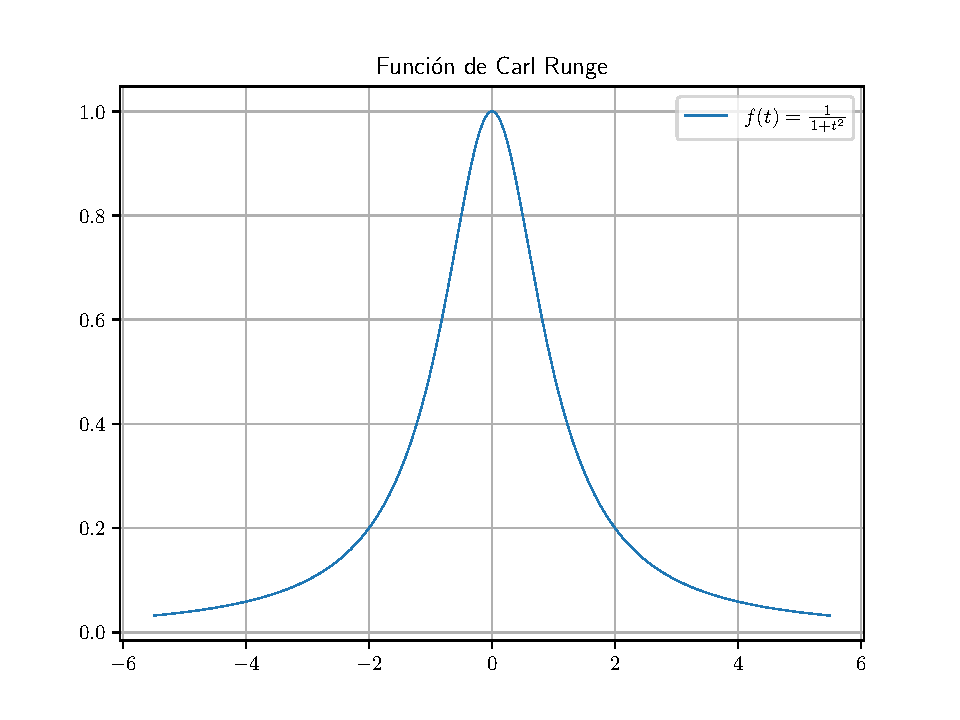
\includegraphics[width=.72\paperwidth]{p12}
        \end{figure}
    \end{solution}
\end{frame}

\begin{frame}
    \begin{solution}
        \begin{equation*}
            P_{4}\left(t\right)=
            0.005305t^{4}-
            0.1711t^{2}+
            5.79\times 10^{-17}t+
            1.
        \end{equation*}
        \begin{figure}[ht!]
            \centering
            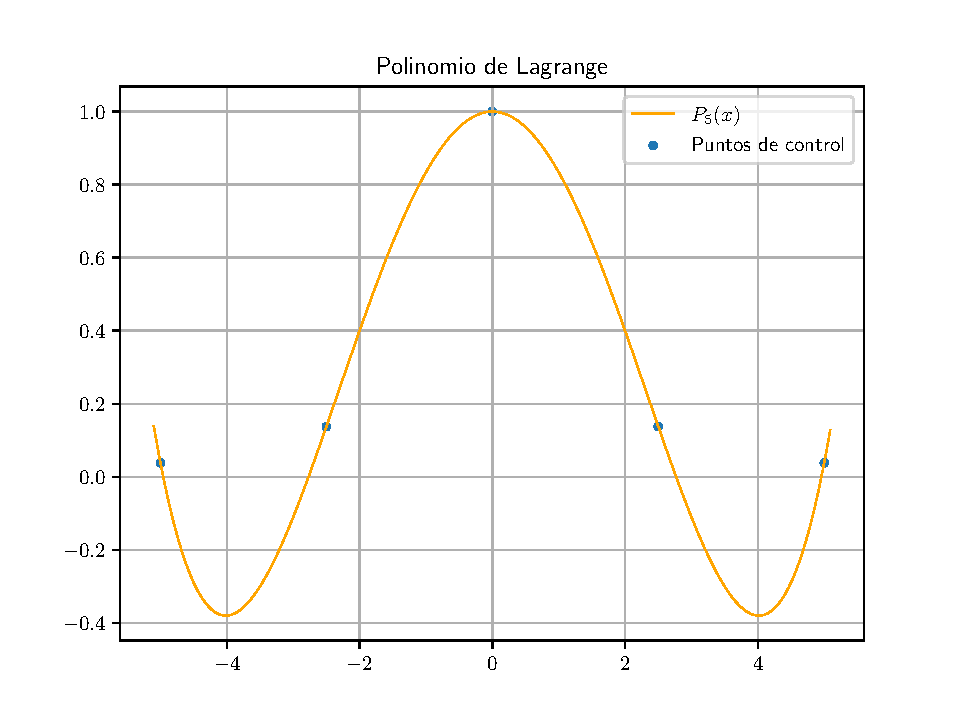
\includegraphics[width=.5\paperwidth]{p12_lagrange5}
        \end{figure}
    \end{solution}
\end{frame}

\begin{frame}
    \begin{solution}
        \begin{equation*}
            P_{7}\left(t\right)=
            3.049\times 10^{-20}t^{7}-
            0.0003311t^{6}+
            2.062\times 10^{-18}t^{5}+
            0.01452t^{4}-
            3.738\times 10^{-17}t^{3}-
            0.1847t^{2}-
            2.46\times 10^{-17}t+
            0.7526.
        \end{equation*}
        \begin{figure}[ht!]
            \centering
            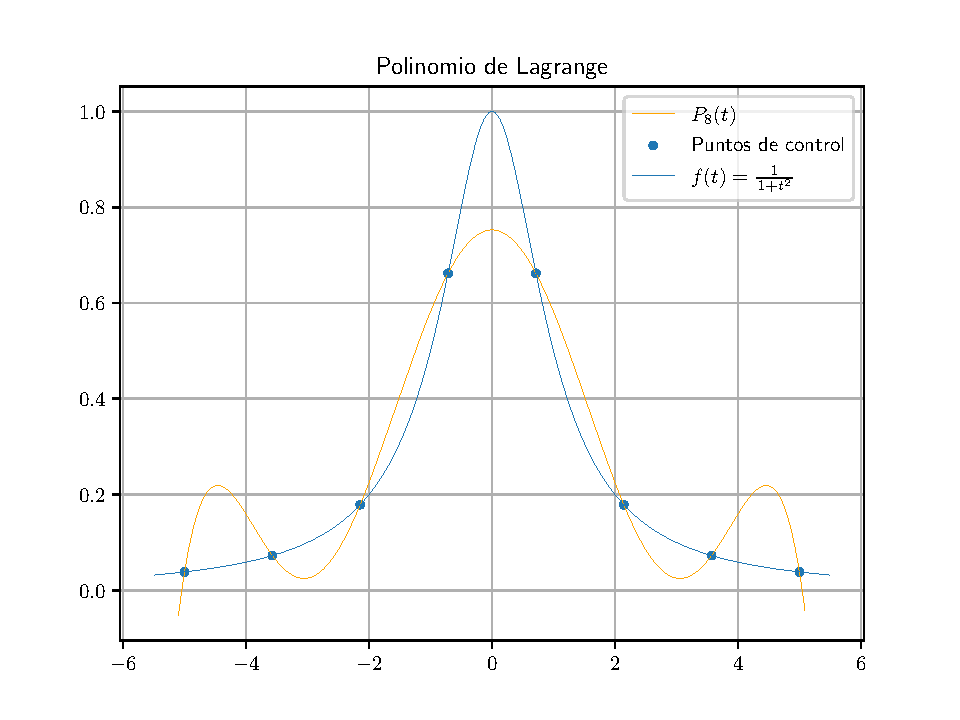
\includegraphics[width=.5\paperwidth]{p12_lagrange8}
        \end{figure}
    \end{solution}
\end{frame}

\begin{frame}
    \begin{solution}
        \begin{equation*}
            P_{9}\left(t\right)=
            -9.099\times 10^{-21}t^{9}+
            5.536\times 10^{-5}t^{8}+
            3.678\times 10^{-19}t^{7}-
            0.002875t^{6}-
            4.312\times 10^{-17}t^{5}+
            0.04917t^{4}+
            6.147\times 10^{-17}t^{3}-
            0.3304t^{2}+
            7.318\times 10^{-17}t+
            0.8615.
        \end{equation*}
        \begin{figure}[ht!]
            \centering
            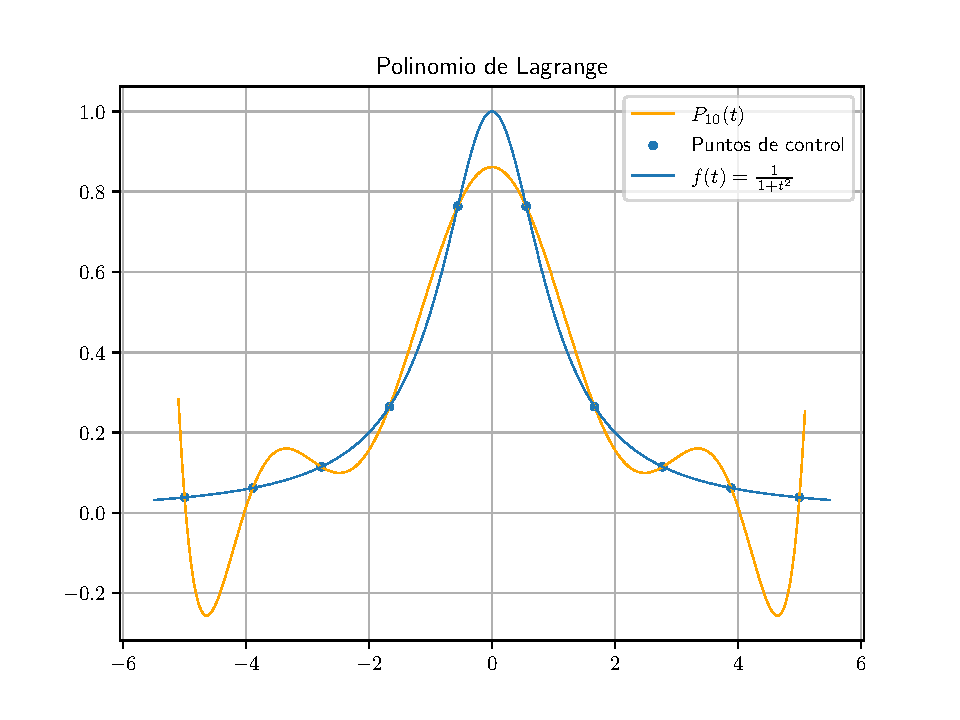
\includegraphics[width=.5\paperwidth]{p12_lagrange10}
        \end{figure}
    \end{solution}
\end{frame}